%%%%%%%%%%%%%%%%%%%%%%%%%%%%%%%%%%%%%%%%%%%%%%%%%%%%%%%%%%%%
% 1.3 ABSTRACT ALGEBRA
% The Composition of Advanced Mathematics
%%%%%%%%%%%%%%%%%%%%%%%%%%%%%%%%%%%%%%%%%%%%%%%%%%%%%%%%%%%%

\section{Abstract Algebra}
\label{sec:abstract-algebra}

\prerequisite{
Elementary set theory from \cref{sec:elementary-set-theory}, relations from
\cref{sec:relations}, functions from \cref{sec:functions}, methods of proof
from \cref{sec:methods-of-proof}, elementary algebra from
\cref{sec:elementary-algebra}, and basic linear algebra from
\cref{sec:linear-algebra}.
}

\learningobjectives{
By the end of this section, the reader should be able to:
\begin{itemize}
    \item explain the structural viewpoint of abstract algebra;
    \item distinguish a set from a set equipped with operations;
    \item interpret unary and binary operations;
    \item test whether an operation is closed;
    \item recognize associativity, commutativity, identities, and inverses;
    \item understand algebraic structures defined by axioms;
    \item distinguish magmas, semigroups, monoids, groups, rings, and fields at an introductory level;
    \item interpret substructures;
    \item understand homomorphisms as structure-preserving functions;
    \item distinguish homomorphisms, isomorphisms, endomorphisms, and automorphisms;
    \item interpret kernels and images structurally;
    \item understand the role of equivalence relations and quotient structures;
    \item recognize generators and cyclic behavior;
    \item interpret operation tables;
    \item understand how symmetries form algebraic structures;
    \item recognize the hierarchy connecting major algebraic systems;
    \item understand why abstract algebra emphasizes structure rather than calculation.
\end{itemize}
}

%%%%%%%%%%%%%%%%%%%%%%%%%%%%%%%%%%%%%%%%%%%%%%%%%%%%%%%%%%%%
\subsection{What Is Abstract Algebra?}
\label{subsec:what-is-abstract-algebra}
%%%%%%%%%%%%%%%%%%%%%%%%%%%%%%%%%%%%%%%%%%%%%%%%%%%%%%%%%%%%

Elementary algebra studies symbolic manipulation involving numbers and
variables.

Abstract algebra asks a different question:

\begin{center}
\emph{What mathematical structures make these manipulations possible?}
\end{center}

For example, ordinary addition of integers satisfies

\[ a+b=b+a. \]

Matrix multiplication generally does not satisfy

\[ AB=BA. \]

Yet both operations have enough structure to support meaningful algebra.

\begin{conceptbox}
Abstract algebra studies sets together with operations and the structural laws
satisfied by those operations.
\end{conceptbox}

The emphasis shifts from particular numbers to patterns shared by many
different mathematical systems.

%%%%%%%%%%%%%%%%%%%%%%%%%%%%%%%%%%%%%%%%%%%%%%%%%%%%%%%%%%%%
\subsection{From Objects to Structures}
\label{subsec:objects-to-structures}
%%%%%%%%%%%%%%%%%%%%%%%%%%%%%%%%%%%%%%%%%%%%%%%%%%%%%%%%%%%%

A set by itself contains elements.

For example,

\[ \Z=\{\ldots,-2,-1,0,1,2,\ldots\}. \]

Once an operation is specified, additional structure appears.

For example,

\[ (\Z,+) \]

means the integers equipped with addition.

Likewise,

\[ (\R,\cdot) \]

means the real numbers equipped with multiplication.

These structures behave differently because the operations satisfy different
properties.

%%%%%%%%%%%%%%%%%%%%%%%%%%%%%%%%%%%%%%%%%%%%%%%%%%%%%%%%%%%%
\subsection{Visualizing Algebraic Structure}
\label{subsec:visualizing-algebraic-structure}
%%%%%%%%%%%%%%%%%%%%%%%%%%%%%%%%%%%%%%%%%%%%%%%%%%%%%%%%%%%%

An algebraic structure can be viewed schematically as

\begin{center}
\begin{tikzpicture}[
    node distance=11mm,
    box/.style={draw,rounded corners,align=center,inner sep=5pt},
    >=stealth
]
\node[box] (set) {Underlying set};
\node[box,right=of set] (op) {Operation};
\node[box,right=of op] (laws) {Axioms and laws};
\node[box,right=of laws] (struct) {Algebraic structure};

\draw[->,thick] (set)--(op);
\draw[->,thick] (op)--(laws);
\draw[->,thick] (laws)--(struct);
\end{tikzpicture}
\end{center}

The same set equipped with a different operation may form a different
algebraic structure.

%%%%%%%%%%%%%%%%%%%%%%%%%%%%%%%%%%%%%%%%%%%%%%%%%%%%%%%%%%%%
\subsection{Operations}
\label{subsec:abstract-operations}
%%%%%%%%%%%%%%%%%%%%%%%%%%%%%%%%%%%%%%%%%%%%%%%%%%%%%%%%%%%%

An operation combines or transforms elements according to a rule.

A \emph{unary operation} acts on one input.

For example,

\[ x\mapsto -x \]

is unary.

A \emph{binary operation} combines two inputs.

For example,

\[ (a,b)\mapsto a+b \]

is binary.

%%%%%%%%%%%%%%%%%%%%%%%%%%%%%%%%%%%%%%%%%%%%%%%%%%%%%%%%%%%%
\subsection{Binary Operations}
\label{subsec:binary-operations}
%%%%%%%%%%%%%%%%%%%%%%%%%%%%%%%%%%%%%%%%%%%%%%%%%%%%%%%%%%%%

\begin{definitionbox}{Binary Operation}
A binary operation on a set \(S\) is a function
\[ *:S\times S\to S. \]
\end{definitionbox}

The symbol

\[ * \]

is read ``star'' and represents a generic binary operation.

The expression

\[ a*b \]

is read ``\(a\) star \(b\).''

The requirement

\[ *:S\times S\to S \]

means that combining two elements of \(S\) must produce another element of
\(S\).

%%%%%%%%%%%%%%%%%%%%%%%%%%%%%%%%%%%%%%%%%%%%%%%%%%%%%%%%%%%%
\subsection{Closure}
\label{subsec:closure-abstract-algebra}
%%%%%%%%%%%%%%%%%%%%%%%%%%%%%%%%%%%%%%%%%%%%%%%%%%%%%%%%%%%%

\begin{definitionbox}{Closure}
A set \(S\) is \emph{closed} under a binary operation \(*\) if
\[ a,b\in S\Longrightarrow a*b\in S. \]
\end{definitionbox}

For example, the integers are closed under addition:

\[ a,b\in\Z\Longrightarrow a+b\in\Z. \]

They are not closed under ordinary division.

For instance,

\[ 1,2\in\Z,\qquad \frac12\notin\Z. \]

%%%%%%%%%%%%%%%%%%%%%%%%%%%%%%%%%%%%%%%%%%%%%%%%%%%%%%%%%%%%
\subsection{Visualizing Closure}
\label{subsec:visual-closure}
%%%%%%%%%%%%%%%%%%%%%%%%%%%%%%%%%%%%%%%%%%%%%%%%%%%%%%%%%%%%

\begin{center}
\begin{tikzpicture}[>=stealth]
\draw (0,0) ellipse (2 and 1.4);
\node at (0,1.8) {\(S\)};
\fill (-0.8,0.3) circle (2pt);
\fill (0.6,0.4) circle (2pt);
\fill (0,-0.5) circle (2pt);

\node[left] at (-0.8,0.3) {\(a\)};
\node[right] at (0.6,0.4) {\(b\)};
\node[below] at (0,-0.5) {\(a*b\)};

\draw[->] (-0.7,0.25) to[bend right=25] (-0.1,-0.4);
\draw[->] (0.5,0.35) to[bend left=25] (0.1,-0.4);

\node at (4,0) {\(\Longrightarrow\)};
\node at (6,0) {\(a*b\in S\)};
\end{tikzpicture}
\end{center}

Closure means the operation never leaves the underlying set.

%%%%%%%%%%%%%%%%%%%%%%%%%%%%%%%%%%%%%%%%%%%%%%%%%%%%%%%%%%%%
\subsection{Associativity}
\label{subsec:associativity-abstract}
%%%%%%%%%%%%%%%%%%%%%%%%%%%%%%%%%%%%%%%%%%%%%%%%%%%%%%%%%%%%

An operation \(*\) is associative if

\[ (a*b)*c=a*(b*c) \]

for all applicable \(a,b,c\).

Associativity concerns the placement of parentheses.

For ordinary addition,

\[ (2+3)+4=2+(3+4). \]

Subtraction is not associative:

\[ (5-3)-1=1, \]

while

\[ 5-(3-1)=3. \]

%%%%%%%%%%%%%%%%%%%%%%%%%%%%%%%%%%%%%%%%%%%%%%%%%%%%%%%%%%%%
\subsection{Commutativity}
\label{subsec:commutativity-abstract}
%%%%%%%%%%%%%%%%%%%%%%%%%%%%%%%%%%%%%%%%%%%%%%%%%%%%%%%%%%%%

An operation is commutative if

\[ a*b=b*a. \]

Commutativity concerns the order of the operands.

Addition of real numbers is commutative.

Matrix multiplication generally is not.

\begin{warningbox}
Associativity and commutativity describe different properties.

Associativity changes grouping:
\[ (a*b)*c=a*(b*c). \]

Commutativity changes order:
\[ a*b=b*a. \]
\end{warningbox}

%%%%%%%%%%%%%%%%%%%%%%%%%%%%%%%%%%%%%%%%%%%%%%%%%%%%%%%%%%%%
\subsection{Identity Elements}
\label{subsec:identity-elements}
%%%%%%%%%%%%%%%%%%%%%%%%%%%%%%%%%%%%%%%%%%%%%%%%%%%%%%%%%%%%

\begin{definitionbox}{Identity Element}
An identity element \(e\in S\) for a binary operation \(*\) satisfies
\[ e*a=a*e=a \]
for every \(a\in S\).
\end{definitionbox}

The symbol \(e\) is commonly used for a generic identity element and is read
``\(e\).''

For addition,

\[ 0+a=a+0=a. \]

Thus \(0\) is the additive identity.

For multiplication,

\[ 1a=a1=a. \]

Thus \(1\) is the multiplicative identity.

%%%%%%%%%%%%%%%%%%%%%%%%%%%%%%%%%%%%%%%%%%%%%%%%%%%%%%%%%%%%
\subsection{Uniqueness of the Identity}
\label{subsec:identity-unique}
%%%%%%%%%%%%%%%%%%%%%%%%%%%%%%%%%%%%%%%%%%%%%%%%%%%%%%%%%%%%

\begin{theorem}
If an identity element exists for a binary operation, it is unique.
\end{theorem}

\begin{proof}
Suppose \(e\) and \(f\) are both identities.

Since \(e\) is an identity,

\[ e*f=f. \]

Since \(f\) is an identity,

\[ e*f=e. \]

Therefore,

\[ e=f. \]
\end{proof}

%%%%%%%%%%%%%%%%%%%%%%%%%%%%%%%%%%%%%%%%%%%%%%%%%%%%%%%%%%%%
\subsection{Inverse Elements}
\label{subsec:inverse-elements}
%%%%%%%%%%%%%%%%%%%%%%%%%%%%%%%%%%%%%%%%%%%%%%%%%%%%%%%%%%%%

\begin{definitionbox}{Inverse Element}
Suppose \(S\) has identity \(e\). An element \(b\in S\) is an inverse of
\(a\in S\) if
\[ a*b=b*a=e. \]
\end{definitionbox}

In multiplicative notation, the inverse of \(a\) is often written

\[ a^{-1}. \]

This is read ``\(a\) inverse.''

In additive notation, the inverse of \(a\) is usually written

\[ -a. \]

%%%%%%%%%%%%%%%%%%%%%%%%%%%%%%%%%%%%%%%%%%%%%%%%%%%%%%%%%%%%
\subsection{Examples of Inverses}
\label{subsec:examples-inverses}
%%%%%%%%%%%%%%%%%%%%%%%%%%%%%%%%%%%%%%%%%%%%%%%%%%%%%%%%%%%%

Under addition in \(\Z\),

\[ 5+(-5)=0. \]

Thus \(-5\) is the additive inverse of \(5\).

Under multiplication in \(\R\setminus\{0\}\),

\[ 5\left(\frac15\right)=1. \]

Thus

\[ \frac15=5^{-1}. \]

%%%%%%%%%%%%%%%%%%%%%%%%%%%%%%%%%%%%%%%%%%%%%%%%%%%%%%%%%%%%
\subsection{Operation Tables}
\label{subsec:operation-tables}
%%%%%%%%%%%%%%%%%%%%%%%%%%%%%%%%%%%%%%%%%%%%%%%%%%%%%%%%%%%%

A finite binary operation can be displayed using an operation table.

For example, consider

\[ S=\{0,1,2\} \]

with addition modulo \(3\).

\[
\begin{array}{c|ccc}
+_3 & 0 & 1 & 2\\
\hline
0 & 0 & 1 & 2\\
1 & 1 & 2 & 0\\
2 & 2 & 0 & 1
\end{array}
\]

The notation

\[ +_3 \]

means addition modulo \(3\).

For example,

\[ 2+_3 2=1. \]

%%%%%%%%%%%%%%%%%%%%%%%%%%%%%%%%%%%%%%%%%%%%%%%%%%%%%%%%%%%%
\subsection{Reading an Operation Table}
\label{subsec:reading-operation-table}
%%%%%%%%%%%%%%%%%%%%%%%%%%%%%%%%%%%%%%%%%%%%%%%%%%%%%%%%%%%%

To compute

\[ 1+_3 2, \]

locate the row labeled \(1\) and column labeled \(2\).

The corresponding entry is

\[ 0. \]

Therefore,

\[ 1+_3 2=0. \]

Operation tables are especially useful for finite groups and other finite
algebraic systems.

%%%%%%%%%%%%%%%%%%%%%%%%%%%%%%%%%%%%%%%%%%%%%%%%%%%%%%%%%%%%
\subsection{A Hierarchy of Algebraic Structures}
\label{subsec:hierarchy-algebraic-structures}
%%%%%%%%%%%%%%%%%%%%%%%%%%%%%%%%%%%%%%%%%%%%%%%%%%%%%%%%%%%%

Different algebraic structures arise by imposing progressively stronger
conditions.

\begin{center}
\begin{tikzpicture}[
    node distance=9mm,
    box/.style={draw,rounded corners,align=center,inner sep=4pt,font=\small},
    >=stealth
]
\node[box] (magma) {Magma\\closure};
\node[box,below=of magma] (semi) {Semigroup\\+ associativity};
\node[box,below=of semi] (monoid) {Monoid\\+ identity};
\node[box,below=of monoid] (group) {Group\\+ inverses};
\node[box,below=of group] (abelian) {Abelian group\\+ commutativity};

\draw[->] (magma)--(semi);
\draw[->] (semi)--(monoid);
\draw[->] (monoid)--(group);
\draw[->] (group)--(abelian);
\end{tikzpicture}
\end{center}

These terms describe increasingly structured binary systems.

%%%%%%%%%%%%%%%%%%%%%%%%%%%%%%%%%%%%%%%%%%%%%%%%%%%%%%%%%%%%
\subsection{Magmas}
\label{subsec:magmas}
%%%%%%%%%%%%%%%%%%%%%%%%%%%%%%%%%%%%%%%%%%%%%%%%%%%%%%%%%%%%

\begin{definitionbox}{Magma}
A \emph{magma} is a set equipped with a closed binary operation.
\end{definitionbox}

No associativity, identity, inverses, or commutativity are required.

This is one of the weakest commonly named algebraic structures.

%%%%%%%%%%%%%%%%%%%%%%%%%%%%%%%%%%%%%%%%%%%%%%%%%%%%%%%%%%%%
\subsection{Semigroups}
\label{subsec:semigroups}
%%%%%%%%%%%%%%%%%%%%%%%%%%%%%%%%%%%%%%%%%%%%%%%%%%%%%%%%%%%%

\begin{definitionbox}{Semigroup}
A \emph{semigroup} is a set equipped with an associative binary operation.
\end{definitionbox}

Thus a semigroup satisfies closure and associativity.

%%%%%%%%%%%%%%%%%%%%%%%%%%%%%%%%%%%%%%%%%%%%%%%%%%%%%%%%%%%%
\subsection{Monoids}
\label{subsec:monoids}
%%%%%%%%%%%%%%%%%%%%%%%%%%%%%%%%%%%%%%%%%%%%%%%%%%%%%%%%%%%%

\begin{definitionbox}{Monoid}
A \emph{monoid} is a semigroup having an identity element.
\end{definitionbox}

For example, the nonnegative integers under addition form a monoid:

\[ (\{0,1,2,\ldots\},+). \]

The identity is \(0\).

Not every element has an additive inverse within this set, so it is not a
group.

%%%%%%%%%%%%%%%%%%%%%%%%%%%%%%%%%%%%%%%%%%%%%%%%%%%%%%%%%%%%
\subsection{Groups}
\label{subsec:groups-overview}
%%%%%%%%%%%%%%%%%%%%%%%%%%%%%%%%%%%%%%%%%%%%%%%%%%%%%%%%%%%%

\begin{definitionbox}{Group}
A \emph{group} is a set \(G\) equipped with a binary operation satisfying:
\begin{enumerate}
    \item closure;
    \item associativity;
    \item existence of an identity;
    \item existence of an inverse for every element.
\end{enumerate}
\end{definitionbox}

If the operation is also commutative, the group is called \emph{abelian}.

Group theory is developed fully in \cref{sec:group-theory}.

%%%%%%%%%%%%%%%%%%%%%%%%%%%%%%%%%%%%%%%%%%%%%%%%%%%%%%%%%%%%
\subsection{Example: Integers under Addition}
\label{subsec:integers-addition-group}
%%%%%%%%%%%%%%%%%%%%%%%%%%%%%%%%%%%%%%%%%%%%%%%%%%%%%%%%%%%%

The structure

\[ (\Z,+) \]

is an abelian group.

Closure:

\[ a,b\in\Z\Longrightarrow a+b\in\Z. \]

Associativity:

\[ (a+b)+c=a+(b+c). \]

Identity:

\[ 0+a=a. \]

Inverse:

\[ a+(-a)=0. \]

Commutativity:

\[ a+b=b+a. \]

%%%%%%%%%%%%%%%%%%%%%%%%%%%%%%%%%%%%%%%%%%%%%%%%%%%%%%%%%%%%
\subsection{Example: Nonzero Real Numbers under Multiplication}
\label{subsec:nonzero-reals-multiplication}
%%%%%%%%%%%%%%%%%%%%%%%%%%%%%%%%%%%%%%%%%%%%%%%%%%%%%%%%%%%%

The structure

\[ (\R\setminus\{0\},\cdot) \]

is also an abelian group.

The identity is

\[ 1. \]

The inverse of \(a\neq0\) is

\[ a^{-1}=\frac1a. \]

%%%%%%%%%%%%%%%%%%%%%%%%%%%%%%%%%%%%%%%%%%%%%%%%%%%%%%%%%%%%
\subsection{Why Zero Is Removed}
\label{subsec:why-zero-removed}
%%%%%%%%%%%%%%%%%%%%%%%%%%%%%%%%%%%%%%%%%%%%%%%%%%%%%%%%%%%%

If \(0\) were included under multiplication, it would need a multiplicative
inverse.

That would require some real \(x\) satisfying

\[ 0x=1. \]

No such real number exists.

Therefore,

\[ (\R,\cdot) \]

is not a group.

%%%%%%%%%%%%%%%%%%%%%%%%%%%%%%%%%%%%%%%%%%%%%%%%%%%%%%%%%%%%
\subsection{Symmetry as Algebra}
\label{subsec:symmetry-as-algebra}
%%%%%%%%%%%%%%%%%%%%%%%%%%%%%%%%%%%%%%%%%%%%%%%%%%%%%%%%%%%%

One of the most important examples of abstract algebra comes from symmetry.

Consider an equilateral triangle.

\begin{center}
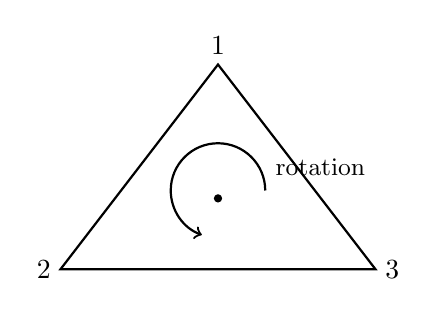
\begin{tikzpicture}[scale=1.0]
\coordinate (A) at (0,2.6);
\coordinate (B) at (-2,0);
\coordinate (C) at (2,0);

\draw[thick] (A)--(B)--(C)--cycle;

\node[above] at (A) {\(1\)};
\node[left] at (B) {\(2\)};
\node[right] at (C) {\(3\)};

\fill (0,0.9) circle (1.5pt);
\draw[->,thick] (0.6,1.0) arc[start angle=0,end angle=250,radius=0.6];
\node at (1.3,1.3) {\small rotation};
\end{tikzpicture}
\end{center}

Rotations and reflections that preserve the triangle can be combined.

The combination of two symmetries is again a symmetry.

These symmetries form a group.

%%%%%%%%%%%%%%%%%%%%%%%%%%%%%%%%%%%%%%%%%%%%%%%%%%%%%%%%%%%%
\subsection{Composition as the Group Operation}
\label{subsec:symmetry-composition}
%%%%%%%%%%%%%%%%%%%%%%%%%%%%%%%%%%%%%%%%%%%%%%%%%%%%%%%%%%%%

For symmetry groups, the operation is function composition.

Suppose \(r\) represents a rotation and \(s\) a reflection.

Then

\[ r\circ s \]

means perform \(s\) first and then \(r\).

Because composition of functions is generally not commutative,

\[ r\circ s\neq s\circ r \]

may occur.

Thus symmetry groups provide natural examples of noncommutative algebra.

%%%%%%%%%%%%%%%%%%%%%%%%%%%%%%%%%%%%%%%%%%%%%%%%%%%%%%%%%%%%
\subsection{Rings}
\label{subsec:rings-overview}
%%%%%%%%%%%%%%%%%%%%%%%%%%%%%%%%%%%%%%%%%%%%%%%%%%%%%%%%%%%%

Groups involve one main binary operation.

Rings introduce two operations, usually called addition and multiplication.

\begin{definitionbox}{Ring}
Informally, a \emph{ring} is a set equipped with addition and multiplication
such that:
\begin{itemize}
    \item addition forms an abelian group;
    \item multiplication is associative;
    \item multiplication distributes over addition.
\end{itemize}
\end{definitionbox}

Precise conventions concerning multiplicative identities vary among texts and
are developed in \cref{sec:ring-theory}.

%%%%%%%%%%%%%%%%%%%%%%%%%%%%%%%%%%%%%%%%%%%%%%%%%%%%%%%%%%%%
\subsection{Example: The Integers as a Ring}
\label{subsec:integers-ring}
%%%%%%%%%%%%%%%%%%%%%%%%%%%%%%%%%%%%%%%%%%%%%%%%%%%%%%%%%%%%

The integers

\[ \Z \]

form a ring under ordinary addition and multiplication.

Addition provides an abelian group.

Multiplication is associative.

The distributive laws hold:

\[ a(b+c)=ab+ac, \]

\[ (a+b)c=ac+bc. \]

%%%%%%%%%%%%%%%%%%%%%%%%%%%%%%%%%%%%%%%%%%%%%%%%%%%%%%%%%%%%
\subsection{Fields}
\label{subsec:fields-overview}
%%%%%%%%%%%%%%%%%%%%%%%%%%%%%%%%%%%%%%%%%%%%%%%%%%%%%%%%%%%%

Fields provide an even richer structure.

\begin{definitionbox}{Field}
A \emph{field} is, informally, a commutative ring in which every nonzero
element has a multiplicative inverse.
\end{definitionbox}

Examples include

\[ \Q,\qquad \R,\qquad \C. \]

The integers \(\Z\) are not a field because most nonzero integers do not have
multiplicative inverses in \(\Z\).

For example,

\[ 2^{-1}=\frac12\notin\Z. \]

Field theory is developed in \cref{sec:field-theory}.

%%%%%%%%%%%%%%%%%%%%%%%%%%%%%%%%%%%%%%%%%%%%%%%%%%%%%%%%%%%%
\subsection{Structural Hierarchy: Groups, Rings, and Fields}
\label{subsec:group-ring-field-hierarchy}
%%%%%%%%%%%%%%%%%%%%%%%%%%%%%%%%%%%%%%%%%%%%%%%%%%%%%%%%%%%%

\begin{center}
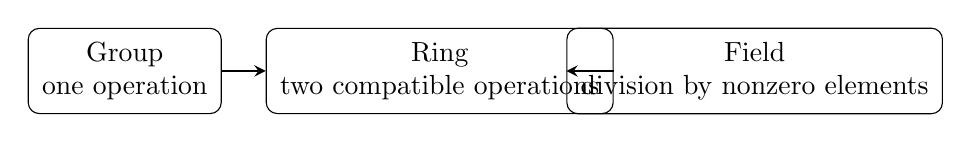
\begin{tikzpicture}[
    node distance=14mm,
    box/.style={draw,rounded corners,align=center,inner sep=5pt},
    >=stealth
]
\node[box] (group) at (0,0) {Group\\one operation};
\node[box] (ring) at (4,0) {Ring\\two compatible operations};
\node[box] (field) at (8,0) {Field\\division by nonzero elements};

\draw[->,thick] (group)--(ring);
\draw[->,thick] (ring)--(field);
\end{tikzpicture}
\end{center}

This diagram is conceptual rather than a literal statement that every group is
a ring or every ring is a field.

Instead, it shows increasing algebraic richness.

%%%%%%%%%%%%%%%%%%%%%%%%%%%%%%%%%%%%%%%%%%%%%%%%%%%%%%%%%%%%
\subsection{Substructures}
\label{subsec:substructures}
%%%%%%%%%%%%%%%%%%%%%%%%%%%%%%%%%%%%%%%%%%%%%%%%%%%%%%%%%%%%

An algebraic structure may contain a smaller subset that inherits the same
type of structure.

Examples include:

\begin{itemize}
    \item subgroups;
    \item subrings;
    \item subfields;
    \item vector subspaces.
\end{itemize}

The general pattern is

\begin{center}
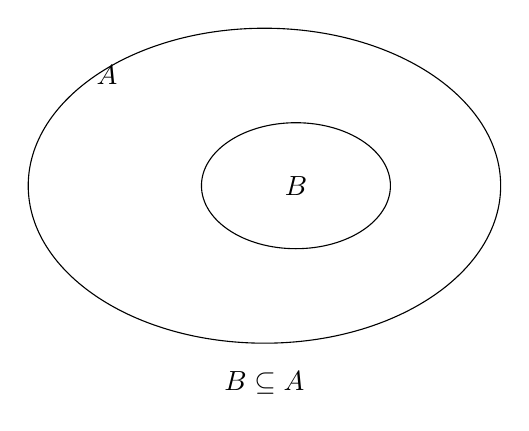
\begin{tikzpicture}
\draw (0,0) ellipse (3 and 2);
\draw (0.4,0) ellipse (1.2 and 0.8);
\node at (-2,1.4) {\(A\)};
\node at (0.4,0) {\(B\)};
\node at (0,-2.5) {\(B\subseteq A\)};
\end{tikzpicture}
\end{center}

The subset must be closed under the relevant operations and satisfy the
necessary axioms.

%%%%%%%%%%%%%%%%%%%%%%%%%%%%%%%%%%%%%%%%%%%%%%%%%%%%%%%%%%%%
\subsection{Generators}
\label{subsec:generators}
%%%%%%%%%%%%%%%%%%%%%%%%%%%%%%%%%%%%%%%%%%%%%%%%%%%%%%%%%%%%

Some structures can be built from a small number of elements.

An element or set of elements from which the entire structure can be produced
is called a \emph{generator} or generating set.

For example, under addition,

\[ \Z=\{\ldots,-2,-1,0,1,2,\ldots\} \]

is generated by \(1\), because every integer can be obtained from repeated
addition of \(1\), together with inverses.

Symbolically,

\[ \Z=\langle 1\rangle. \]

The angle-bracket notation

\[ \langle 1\rangle \]

is read ``the structure generated by \(1\)'' or, in group theory, ``the group
generated by \(1\).''

%%%%%%%%%%%%%%%%%%%%%%%%%%%%%%%%%%%%%%%%%%%%%%%%%%%%%%%%%%%%
\subsection{Cyclic Structure}
\label{subsec:cyclic-structure}
%%%%%%%%%%%%%%%%%%%%%%%%%%%%%%%%%%%%%%%%%%%%%%%%%%%%%%%%%%%%

A group generated by a single element is called \emph{cyclic}.

The finite cyclic structure with four elements can be visualized as

\begin{center}
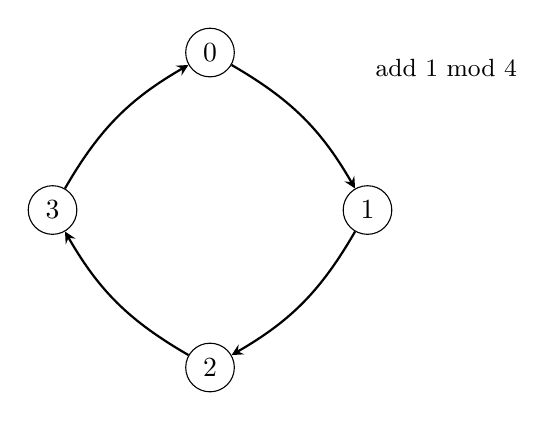
\begin{tikzpicture}[>=stealth]
\node[circle,draw] (0) at (0,2) {\(0\)};
\node[circle,draw] (1) at (2,0) {\(1\)};
\node[circle,draw] (2) at (0,-2) {\(2\)};
\node[circle,draw] (3) at (-2,0) {\(3\)};

\draw[->,thick] (0) to[bend left=15] (1);
\draw[->,thick] (1) to[bend left=15] (2);
\draw[->,thick] (2) to[bend left=15] (3);
\draw[->,thick] (3) to[bend left=15] (0);

\node at (3,1.8) {\small add \(1\) mod \(4\)};
\end{tikzpicture}
\end{center}

Repeated application of the generator eventually reaches every element.

%%%%%%%%%%%%%%%%%%%%%%%%%%%%%%%%%%%%%%%%%%%%%%%%%%%%%%%%%%%%
\subsection{Homomorphisms}
\label{subsec:homomorphisms}
%%%%%%%%%%%%%%%%%%%%%%%%%%%%%%%%%%%%%%%%%%%%%%%%%%%%%%%%%%%%

A major goal of abstract algebra is to compare structures.

The appropriate maps are those that preserve operations.

\begin{definitionbox}{Homomorphism}
A \emph{homomorphism} is a function between algebraic structures that preserves
the relevant operations.
\end{definitionbox}

For structures with operation \(*\), a homomorphism \(\varphi\) typically
satisfies

\[ \varphi(a*b)=\varphi(a)*\varphi(b). \]

The symbol

\[ \varphi \]

is lowercase Greek \emph{phi}, commonly pronounced ``fie'' or ``fee.''

%%%%%%%%%%%%%%%%%%%%%%%%%%%%%%%%%%%%%%%%%%%%%%%%%%%%%%%%%%%%
\subsection{Visualizing a Homomorphism}
\label{subsec:visual-homomorphism}
%%%%%%%%%%%%%%%%%%%%%%%%%%%%%%%%%%%%%%%%%%%%%%%%%%%%%%%%%%%%

\begin{center}
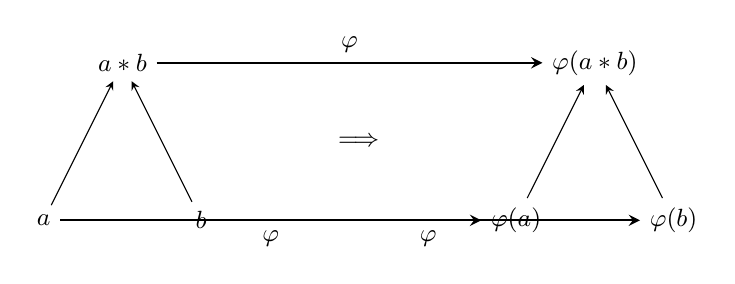
\begin{tikzpicture}[
    node distance=16mm,
    >=stealth,
    every node/.style={font=\small}
]
\node (ab) at (0,2) {\(a*b\)};
\node (a) at (-1,0) {\(a\)};
\node (b) at (1,0) {\(b\)};

\node (fab) at (6,2) {\(\varphi(a*b)\)};
\node (fa) at (5,0) {\(\varphi(a)\)};
\node (fb) at (7,0) {\(\varphi(b)\)};

\draw[->] (a)--(ab);
\draw[->] (b)--(ab);
\draw[->,thick] (ab)--node[above]{\(\varphi\)}(fab);
\draw[->,thick] (a)--node[below]{\(\varphi\)}(fa);
\draw[->,thick] (b)--node[below]{\(\varphi\)}(fb);
\draw[->] (fa)--(fab);
\draw[->] (fb)--(fab);

\node at (3,1) {\(\Longrightarrow\)};
\end{tikzpicture}
\end{center}

The essential principle is:

\begin{center}
\emph{combine first and map, or map first and combine; the result is the same.}
\end{center}

%%%%%%%%%%%%%%%%%%%%%%%%%%%%%%%%%%%%%%%%%%%%%%%%%%%%%%%%%%%%
\subsection{Example of a Homomorphism}
\label{subsec:homomorphism-example}
%%%%%%%%%%%%%%%%%%%%%%%%%%%%%%%%%%%%%%%%%%%%%%%%%%%%%%%%%%%%

Consider

\[ \varphi:\Z\to\Z_n \]

defined by

\[ \varphi(k)=[k]_n, \]

where \([k]_n\) denotes the congruence class of \(k\) modulo \(n\).

Then

\[ \varphi(a+b)=[a+b]_n. \]

Also,

\[ \varphi(a)+\varphi(b)=[a]_n+[b]_n=[a+b]_n. \]

Therefore,

\[ \varphi(a+b)=\varphi(a)+\varphi(b). \]

Thus \(\varphi\) preserves addition.

%%%%%%%%%%%%%%%%%%%%%%%%%%%%%%%%%%%%%%%%%%%%%%%%%%%%%%%%%%%%
\subsection{Isomorphisms}
\label{subsec:isomorphisms}
%%%%%%%%%%%%%%%%%%%%%%%%%%%%%%%%%%%%%%%%%%%%%%%%%%%%%%%%%%%%

\begin{definitionbox}{Isomorphism}
An \emph{isomorphism} is a bijective homomorphism.
\end{definitionbox}

Two structures connected by an isomorphism are called \emph{isomorphic}.

The notation

\[ A\cong B \]

is read ``\(A\) is isomorphic to \(B\).''

The symbol

\[ \cong \]

is called an \emph{isomorphism symbol} in this context and is read ``is
isomorphic to.''

%%%%%%%%%%%%%%%%%%%%%%%%%%%%%%%%%%%%%%%%%%%%%%%%%%%%%%%%%%%%
\subsection{What Isomorphism Means}
\label{subsec:meaning-isomorphism}
%%%%%%%%%%%%%%%%%%%%%%%%%%%%%%%%%%%%%%%%%%%%%%%%%%%%%%%%%%%%

Isomorphic structures may contain different types of objects but have the same
algebraic structure.

\begin{center}
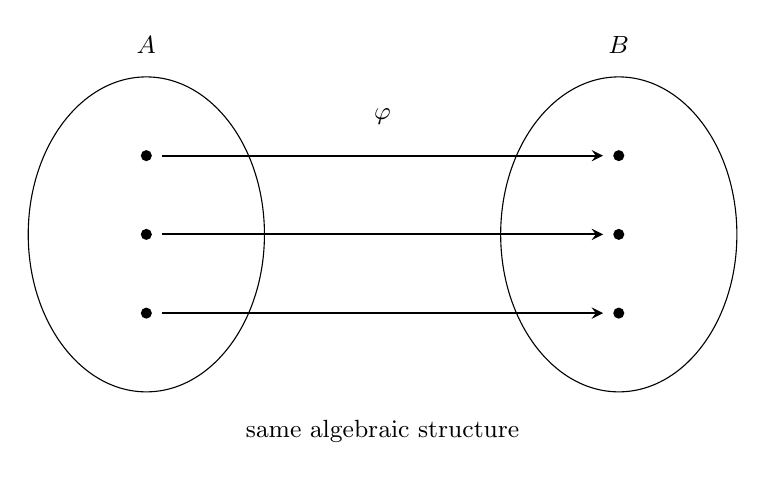
\begin{tikzpicture}[
    >=stealth,
    every node/.style={font=\small}
]
\draw (-2,0) ellipse (1.5 and 2);
\draw (4,0) ellipse (1.5 and 2);

\node at (-2,2.4) {\(A\)};
\node at (4,2.4) {\(B\)};

\fill (-2,1) circle (2pt);
\fill (-2,0) circle (2pt);
\fill (-2,-1) circle (2pt);

\fill (4,1) circle (2pt);
\fill (4,0) circle (2pt);
\fill (4,-1) circle (2pt);

\draw[->,thick] (-1.8,1)--(3.8,1);
\draw[->,thick] (-1.8,0)--(3.8,0);
\draw[->,thick] (-1.8,-1)--(3.8,-1);

\node at (1,1.5) {\(\varphi\)};
\node at (1,-2.5) {same algebraic structure};
\end{tikzpicture}
\end{center}

From the viewpoint of abstract algebra, isomorphic structures are often
treated as structurally identical.

%%%%%%%%%%%%%%%%%%%%%%%%%%%%%%%%%%%%%%%%%%%%%%%%%%%%%%%%%%%%
\subsection{Endomorphisms and Automorphisms}
\label{subsec:endomorphisms-automorphisms}
%%%%%%%%%%%%%%%%%%%%%%%%%%%%%%%%%%%%%%%%%%%%%%%%%%%%%%%%%%%%

A homomorphism from a structure to itself is called an \emph{endomorphism}.

Thus,

\[ \varphi:A\to A. \]

An isomorphism from a structure to itself is called an \emph{automorphism}.

Automorphisms describe internal symmetries of algebraic structures.

%%%%%%%%%%%%%%%%%%%%%%%%%%%%%%%%%%%%%%%%%%%%%%%%%%%%%%%%%%%%
\subsection{Kernel of a Homomorphism}
\label{subsec:kernel-homomorphism}
%%%%%%%%%%%%%%%%%%%%%%%%%%%%%%%%%%%%%%%%%%%%%%%%%%%%%%%%%%%%

For group-like structures, the kernel consists of elements mapped to the
identity.

If

\[ \varphi:G\to H, \]

then

\[ \Ker(\varphi)=\{g\in G:\varphi(g)=e_H\}. \]

The notation \(e_H\) denotes the identity element of \(H\).

The kernel measures how much information the homomorphism collapses.

%%%%%%%%%%%%%%%%%%%%%%%%%%%%%%%%%%%%%%%%%%%%%%%%%%%%%%%%%%%%
\subsection{Image of a Homomorphism}
\label{subsec:image-homomorphism}
%%%%%%%%%%%%%%%%%%%%%%%%%%%%%%%%%%%%%%%%%%%%%%%%%%%%%%%%%%%%

The image is

\[ \Image(\varphi)=\{\varphi(g):g\in G\}. \]

It consists of all elements in the target structure that are actually reached.

The kernel and image generalize ideas already encountered in linear algebra.

%%%%%%%%%%%%%%%%%%%%%%%%%%%%%%%%%%%%%%%%%%%%%%%%%%%%%%%%%%%%
\subsection{Structure-Preserving Maps Across Mathematics}
\label{subsec:structure-preserving-maps}
%%%%%%%%%%%%%%%%%%%%%%%%%%%%%%%%%%%%%%%%%%%%%%%%%%%%%%%%%%%%

The same general idea appears throughout mathematics:

\[
\begin{array}{c|c}
\text{Structure} & \text{Structure-preserving map}\\
\hline
\text{sets} & \text{functions}\\
\text{groups} & \text{group homomorphisms}\\
\text{rings} & \text{ring homomorphisms}\\
\text{vector spaces} & \text{linear transformations}\\
\text{topological spaces} & \text{continuous maps}\\
\text{metric spaces} & \text{isometries or continuous maps}
\end{array}
\]

This theme becomes central throughout advanced mathematics.

%%%%%%%%%%%%%%%%%%%%%%%%%%%%%%%%%%%%%%%%%%%%%%%%%%%%%%%%%%%%
\subsection{Equivalence Relations Revisited}
\label{subsec:equivalence-relations-algebra}
%%%%%%%%%%%%%%%%%%%%%%%%%%%%%%%%%%%%%%%%%%%%%%%%%%%%%%%%%%%%

Equivalence relations from \cref{sec:relations} play a major role in abstract
algebra.

Recall that an equivalence relation is:

\begin{itemize}
    \item reflexive;
    \item symmetric;
    \item transitive.
\end{itemize}

An equivalence relation partitions a set into equivalence classes.

%%%%%%%%%%%%%%%%%%%%%%%%%%%%%%%%%%%%%%%%%%%%%%%%%%%%%%%%%%%%
\subsection{Equivalence Classes}
\label{subsec:equivalence-classes-algebra}
%%%%%%%%%%%%%%%%%%%%%%%%%%%%%%%%%%%%%%%%%%%%%%%%%%%%%%%%%%%%

If \(a\in S\), its equivalence class is

\[ [a]=\{x\in S:x\sim a\}. \]

The symbol

\[ \sim \]

is read ``is equivalent to'' in this context.

For congruence modulo \(n\),

\[ [a]_n \]

contains all integers congruent to \(a\) modulo \(n\).

%%%%%%%%%%%%%%%%%%%%%%%%%%%%%%%%%%%%%%%%%%%%%%%%%%%%%%%%%%%%
\subsection{Visualizing Equivalence Classes}
\label{subsec:visual-equivalence-classes}
%%%%%%%%%%%%%%%%%%%%%%%%%%%%%%%%%%%%%%%%%%%%%%%%%%%%%%%%%%%%

\begin{center}
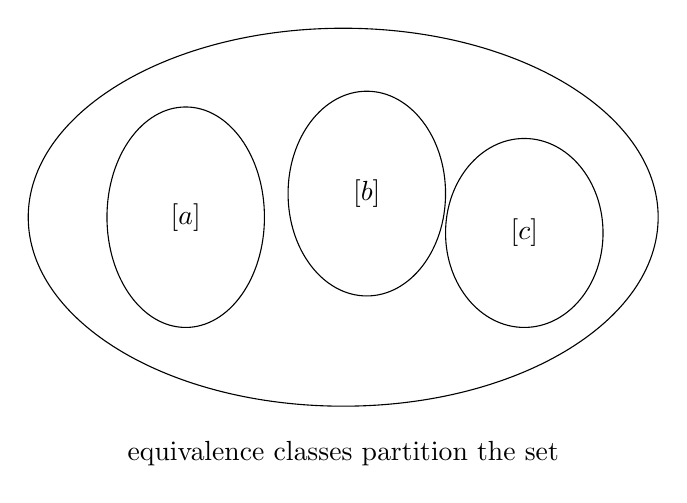
\begin{tikzpicture}
\draw (0,0) ellipse (4 and 2.4);
\draw (-2,0) ellipse (1 and 1.4);
\draw (0.3,0.3) ellipse (1 and 1.3);
\draw (2.3,-0.2) ellipse (1 and 1.2);

\node at (-2,0) {\([a]\)};
\node at (0.3,0.3) {\([b]\)};
\node at (2.3,-0.2) {\([c]\)};
\node at (0,-3) {equivalence classes partition the set};
\end{tikzpicture}
\end{center}

Distinct equivalence classes do not overlap, and together they cover the entire
set.

%%%%%%%%%%%%%%%%%%%%%%%%%%%%%%%%%%%%%%%%%%%%%%%%%%%%%%%%%%%%
\subsection{Quotient Structures}
\label{subsec:quotient-structures}
%%%%%%%%%%%%%%%%%%%%%%%%%%%%%%%%%%%%%%%%%%%%%%%%%%%%%%%%%%%%

A quotient structure replaces individual elements by equivalence classes.

If \(S\) is partitioned by an equivalence relation \(\sim\), then the quotient
set is written

\[ S/{\sim}. \]

This is read

\begin{center}
``\(S\) modulo the equivalence relation \(\sim\)''
\end{center}

or simply

\begin{center}
``\(S\) quotient by \(\sim\).''
\end{center}

%%%%%%%%%%%%%%%%%%%%%%%%%%%%%%%%%%%%%%%%%%%%%%%%%%%%%%%%%%%%
\subsection{Integers Modulo \(n\)}
\label{subsec:integers-mod-n}
%%%%%%%%%%%%%%%%%%%%%%%%%%%%%%%%%%%%%%%%%%%%%%%%%%%%%%%%%%%%

One of the most important quotient constructions is

\[ \Z/n\Z. \]

This is read

\begin{center}
``the integers modulo \(n\)''
\end{center}

or

\begin{center}
``Z mod \(n\) Z.''
\end{center}

Its elements can be represented by congruence classes

\[ [0]_n,[1]_n,\ldots,[n-1]_n. \]

%%%%%%%%%%%%%%%%%%%%%%%%%%%%%%%%%%%%%%%%%%%%%%%%%%%%%%%%%%%%
\subsection{Visualizing Arithmetic Modulo \(n\)}
\label{subsec:visual-modular-arithmetic}
%%%%%%%%%%%%%%%%%%%%%%%%%%%%%%%%%%%%%%%%%%%%%%%%%%%%%%%%%%%%

For arithmetic modulo \(6\), the values wrap around a cycle.

\begin{center}
\begin{tikzpicture}[scale=1.0,>=stealth]
\foreach \k in {0,...,5}{
    \node[circle,draw] (n\k) at ({90-60*\k}:2) {\(\k\)};
}

\foreach \k [evaluate=\k as \next using int(mod(\k+1,6))] in {0,...,5}{
    \draw[->,thick] (n\k) to[bend left=15] (n\next);
}

\node at (4,0) {add \(1\) mod \(6\)};
\end{tikzpicture}
\end{center}

After \(5\), adding \(1\) returns to \(0\).

%%%%%%%%%%%%%%%%%%%%%%%%%%%%%%%%%%%%%%%%%%%%%%%%%%%%%%%%%%%%
\subsection{Well-Defined Operations}
\label{subsec:well-defined-operations}
%%%%%%%%%%%%%%%%%%%%%%%%%%%%%%%%%%%%%%%%%%%%%%%%%%%%%%%%%%%%

When operations are defined on equivalence classes, one must verify that the
result does not depend on the representative chosen.

This property is called \emph{well-definedness}.

Suppose

\[ [a]=[a'] \]

and

\[ [b]=[b']. \]

For an operation on classes to be well defined, we require

\[ [a*b]=[a'*b']. \]

This issue becomes fundamental in quotient groups, quotient rings, and other
quotient structures.

%%%%%%%%%%%%%%%%%%%%%%%%%%%%%%%%%%%%%%%%%%%%%%%%%%%%%%%%%%%%
\subsection{Worked Example: Checking Closure}
\label{subsec:worked-checking-closure}
%%%%%%%%%%%%%%%%%%%%%%%%%%%%%%%%%%%%%%%%%%%%%%%%%%%%%%%%%%%%

\begin{workedexamplebox}{Check Closure}

Determine whether the odd integers are closed under addition.

Let

\[ a=2m+1,\qquad b=2n+1 \]

be odd integers.

\begin{tabularx}{\textwidth}{@{}>{\raggedright\arraybackslash}p{0.42\textwidth}X@{}}
Add the two numbers. & \(a+b=2m+1+2n+1\)\\
Simplify. & \(a+b=2(m+n+1)\)\\
Interpret the result. & The sum is even.
\end{tabularx}

\begin{answerbox}
The odd integers are not closed under addition.
\end{answerbox}
\end{workedexamplebox}

%%%%%%%%%%%%%%%%%%%%%%%%%%%%%%%%%%%%%%%%%%%%%%%%%%%%%%%%%%%%
\subsection{Worked Example: Identity Element}
\label{subsec:worked-identity}
%%%%%%%%%%%%%%%%%%%%%%%%%%%%%%%%%%%%%%%%%%%%%%%%%%%%%%%%%%%%

\begin{workedexamplebox}{Find an Identity Element}

Define an operation on \(\R\) by

\[ a*b=a+b+2. \]

Find the identity.

Let \(e\) satisfy

\[ a*e=a. \]

\begin{tabularx}{\textwidth}{@{}>{\raggedright\arraybackslash}p{0.42\textwidth}X@{}}
Use the operation. & \(a+e+2=a\)\\
Subtract \(a\). & \(e+2=0\)\\
Solve. & \(e=-2\)
\end{tabularx}

Check:

\[ a*(-2)=a-2+2=a. \]

\begin{answerbox}
\[ e=-2 \]
\end{answerbox}
\end{workedexamplebox}

%%%%%%%%%%%%%%%%%%%%%%%%%%%%%%%%%%%%%%%%%%%%%%%%%%%%%%%%%%%%
\subsection{Worked Example: Finding an Inverse}
\label{subsec:worked-inverse-abstract}
%%%%%%%%%%%%%%%%%%%%%%%%%%%%%%%%%%%%%%%%%%%%%%%%%%%%%%%%%%%%

\begin{workedexamplebox}{Find an Inverse under a Custom Operation}

Using

\[ a*b=a+b+2, \]

find the inverse of \(a\).

The identity is

\[ e=-2. \]

Let \(b\) be the inverse of \(a\).

\begin{tabularx}{\textwidth}{@{}>{\raggedright\arraybackslash}p{0.42\textwidth}X@{}}
Require \(a*b=e\). & \(a+b+2=-2\)\\
Solve for \(b\). & \(b=-a-4\)
\end{tabularx}

\begin{answerbox}
The inverse of \(a\) under \(*\) is
\[ -a-4. \]
\end{answerbox}
\end{workedexamplebox}

%%%%%%%%%%%%%%%%%%%%%%%%%%%%%%%%%%%%%%%%%%%%%%%%%%%%%%%%%%%%
\subsection{Why Axioms Matter}
\label{subsec:why-axioms-matter}
%%%%%%%%%%%%%%%%%%%%%%%%%%%%%%%%%%%%%%%%%%%%%%%%%%%%%%%%%%%%

An axiom is not merely a technical condition.

Axioms determine what conclusions are available.

For example:

\begin{itemize}
    \item associativity allows parentheses to be omitted safely in repeated products;
    \item identity elements provide neutral operations;
    \item inverses allow equations to be undone;
    \item distributivity connects two different operations;
    \item commutativity permits factors or terms to be reordered.
\end{itemize}

Changing the axioms changes the mathematics.

%%%%%%%%%%%%%%%%%%%%%%%%%%%%%%%%%%%%%%%%%%%%%%%%%%%%%%%%%%%%
\subsection{Structural Reasoning}
\label{subsec:structural-reasoning}
%%%%%%%%%%%%%%%%%%%%%%%%%%%%%%%%%%%%%%%%%%%%%%%%%%%%%%%%%%%%

Suppose \(G\) is a group and

\[ ab=ac. \]

Elementary algebra may tempt us to ``cancel \(a\).''

Abstract algebra asks why cancellation is valid.

Multiply on the left by \(a^{-1}\):

\[ a^{-1}(ab)=a^{-1}(ac). \]

Associativity gives

\[ (a^{-1}a)b=(a^{-1}a)c. \]

Since

\[ a^{-1}a=e, \]

we obtain

\[ eb=ec. \]

Therefore,

\[ b=c. \]

Cancellation is thus a consequence of the group axioms.

%%%%%%%%%%%%%%%%%%%%%%%%%%%%%%%%%%%%%%%%%%%%%%%%%%%%%%%%%%%%
\subsection{Worked Proof: Uniqueness of Inverses}
\label{subsec:uniqueness-inverses}
%%%%%%%%%%%%%%%%%%%%%%%%%%%%%%%%%%%%%%%%%%%%%%%%%%%%%%%%%%%%

\begin{theorem}
An element of a group has a unique inverse.
\end{theorem}

\begin{proof}
Let \(a\in G\).

Suppose \(b\) and \(c\) are both inverses of \(a\).

Then

\[ ab=e,\qquad ca=e. \]

Now

\[
\begin{aligned}
b
&=be\\
&=b(ac)\\
&=(ba)c\\
&=ec\\
&=c.
\end{aligned}
\]

Therefore the inverse is unique.
\end{proof}

%%%%%%%%%%%%%%%%%%%%%%%%%%%%%%%%%%%%%%%%%%%%%%%%%%%%%%%%%%%%
\subsection{Abstract Algebra and Linear Algebra}
\label{subsec:abstract-linear-connection}
%%%%%%%%%%%%%%%%%%%%%%%%%%%%%%%%%%%%%%%%%%%%%%%%%%%%%%%%%%%%

Linear algebra is already an example of abstract algebra.

A vector space consists of:

\begin{itemize}
    \item a set of vectors;
    \item vector addition;
    \item scalar multiplication;
    \item axioms governing those operations.
\end{itemize}

Linear transformations are structure-preserving maps between vector spaces.

Thus the pattern

\begin{center}
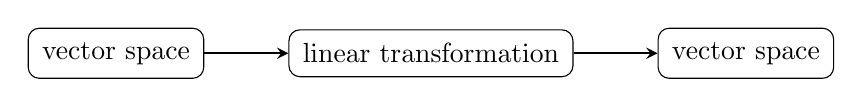
\begin{tikzpicture}[
    box/.style={draw,rounded corners,align=center,inner sep=5pt},
    >=stealth
]
\node[box] (space) at (0,0) {vector space};
\node[box] (map) at (4,0) {linear transformation};
\node[box] (space2) at (8,0) {vector space};

\draw[->,thick] (space)--(map);
\draw[->,thick] (map)--(space2);
\end{tikzpicture}
\end{center}

is a special case of the broader algebraic pattern

\begin{center}
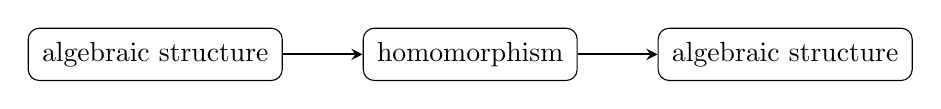
\begin{tikzpicture}[
    box/.style={draw,rounded corners,align=center,inner sep=5pt},
    >=stealth
]
\node[box] (struct) at (0,0) {algebraic structure};
\node[box] (hom) at (4,0) {homomorphism};
\node[box] (struct2) at (8,0) {algebraic structure};

\draw[->,thick] (struct)--(hom);
\draw[->,thick] (hom)--(struct2);
\end{tikzpicture}
\end{center}

%%%%%%%%%%%%%%%%%%%%%%%%%%%%%%%%%%%%%%%%%%%%%%%%%%%%%%%%%%%%
\subsection{Abstract Algebra as a Unifying Language}
\label{subsec:abstract-algebra-unifying}
%%%%%%%%%%%%%%%%%%%%%%%%%%%%%%%%%%%%%%%%%%%%%%%%%%%%%%%%%%%%

Several recurring ideas appear across nearly all areas of algebra.

\[
\begin{array}{c|c}
\text{Idea} & \text{Question}\\
\hline
\text{operation} & \text{How are elements combined?}\\
\text{closure} & \text{Does the operation stay inside the set?}\\
\text{identity} & \text{Is there a neutral element?}\\
\text{inverse} & \text{Can an operation be undone?}\\
\text{substructure} & \text{Does a smaller structure live inside?}\\
\text{generator} & \text{Can the structure be built from a few elements?}\\
\text{homomorphism} & \text{How can structures be compared?}\\
\text{kernel} & \text{What information is collapsed?}\\
\text{image} & \text{What outputs are reached?}\\
\text{quotient} & \text{What happens when equivalent elements are identified?}
\end{array}
\]

These ideas recur in group theory, ring theory, field theory, module theory,
representation theory, topology, and beyond.

%%%%%%%%%%%%%%%%%%%%%%%%%%%%%%%%%%%%%%%%%%%%%%%%%%%%%%%%%%%%
\subsection{Common Abstract Algebra Errors}
\label{subsec:common-abstract-algebra-errors}
%%%%%%%%%%%%%%%%%%%%%%%%%%%%%%%%%%%%%%%%%%%%%%%%%%%%%%%%%%%%

\subsubsection{Assuming Familiar Arithmetic Laws Always Hold}

A new operation may fail to be commutative or associative.

Never assume a property without verifying it or using an axiom that guarantees
it.

%%%%%%%%%%%%%%%%%%%%%%%%%%%%%%%%%%%%%%%%%%%%%%%%%%%%%%%%%%%%
\subsubsection{Confusing Closure with Associativity}
\label{subsec:error-closure-associativity}
%%%%%%%%%%%%%%%%%%%%%%%%%%%%%%%%%%%%%%%%%%%%%%%%%%%%%%%%%%%%

Closure means

\[ a,b\in S\Longrightarrow a*b\in S. \]

Associativity means

\[ (a*b)*c=a*(b*c). \]

They are unrelated conditions.

%%%%%%%%%%%%%%%%%%%%%%%%%%%%%%%%%%%%%%%%%%%%%%%%%%%%%%%%%%%%
\subsubsection{Assuming an Identity Is Always \(0\) or \(1\)}
\label{subsec:error-identity-zero-one}
%%%%%%%%%%%%%%%%%%%%%%%%%%%%%%%%%%%%%%%%%%%%%%%%%%%%%%%%%%%%

The identity depends on the operation.

For

\[ a*b=a+b+2, \]

the identity is

\[ -2. \]

%%%%%%%%%%%%%%%%%%%%%%%%%%%%%%%%%%%%%%%%%%%%%%%%%%%%%%%%%%%%
\subsubsection{Assuming Every Element Has an Inverse}
\label{subsec:error-every-element-inverse}
%%%%%%%%%%%%%%%%%%%%%%%%%%%%%%%%%%%%%%%%%%%%%%%%%%%%%%%%%%%%

Inverse existence depends on the structure.

For example, \(2\) has no multiplicative inverse in \(\Z\).

%%%%%%%%%%%%%%%%%%%%%%%%%%%%%%%%%%%%%%%%%%%%%%%%%%%%%%%%%%%%
\subsubsection{Confusing Homomorphism and Isomorphism}
\label{subsec:error-homomorphism-isomorphism}
%%%%%%%%%%%%%%%%%%%%%%%%%%%%%%%%%%%%%%%%%%%%%%%%%%%%%%%%%%%%

A homomorphism preserves structure.

An isomorphism preserves structure and is bijective.

Every isomorphism is a homomorphism, but not every homomorphism is an
isomorphism.

%%%%%%%%%%%%%%%%%%%%%%%%%%%%%%%%%%%%%%%%%%%%%%%%%%%%%%%%%%%%
\subsubsection{Treating Isomorphic Structures as Literally Equal}
\label{subsec:error-isomorphic-equal}
%%%%%%%%%%%%%%%%%%%%%%%%%%%%%%%%%%%%%%%%%%%%%%%%%%%%%%%%%%%%

If

\[ A\cong B, \]

the structures need not contain the same elements.

They have the same structural form.

%%%%%%%%%%%%%%%%%%%%%%%%%%%%%%%%%%%%%%%%%%%%%%%%%%%%%%%%%%%%
\subsubsection{Ignoring Well-Definedness}
\label{subsec:error-well-definedness}
%%%%%%%%%%%%%%%%%%%%%%%%%%%%%%%%%%%%%%%%%%%%%%%%%%%%%%%%%%%%

A rule involving equivalence classes must give the same result regardless of
which representative is chosen.

Otherwise the operation is not well defined.

%%%%%%%%%%%%%%%%%%%%%%%%%%%%%%%%%%%%%%%%%%%%%%%%%%%%%%%%%%%%
\subsection{Exercises}
\label{subsec:abstract-algebra-exercises}
%%%%%%%%%%%%%%%%%%%%%%%%%%%%%%%%%%%%%%%%%%%%%%%%%%%%%%%%%%%%

\begin{exercise}[1]
Determine whether the integers are closed under subtraction.
\end{exercise}

\begin{exercise}[1]
Determine whether the natural numbers are closed under subtraction.
\end{exercise}

\begin{exercise}[1]
Determine whether the nonzero real numbers are closed under multiplication.
\end{exercise}

\begin{exercise}[1]
Determine whether subtraction on \(\R\) is associative.
\end{exercise}

\begin{exercise}[1]
Determine whether subtraction on \(\R\) is commutative.
\end{exercise}

\begin{exercise}[1]
Identify the identity element of
\[ (\Z,+). \]
\end{exercise}

\begin{exercise}[1]
Find the inverse of \(7\) in
\[ (\Z,+). \]
\end{exercise}

\begin{exercise}[1]
Find the inverse of \(5\) in
\[ (\R\setminus\{0\},\cdot). \]
\end{exercise}

\begin{exercise}[2]
Define
\[ a*b=a+b-3 \]
on \(\R\). Find the identity element.
\end{exercise}

\begin{exercise}[2]
Using
\[ a*b=a+b-3, \]
find the inverse of an arbitrary \(a\in\R\).
\end{exercise}

\begin{exercise}[2]
Determine whether
\[ a*b=a+b+ab \]
is commutative on \(\R\).
\end{exercise}

\begin{exercise}[2]
Determine whether
\[ a*b=a-b \]
defines an associative operation on \(\R\).
\end{exercise}

\begin{exercise}[2]
Construct the operation table for addition modulo \(4\).
\end{exercise}

\begin{exercise}[2]
Using addition modulo \(5\), compute
\[ [3]_5+[4]_5. \]
\end{exercise}

\begin{exercise}[1]
Explain why
\[ (\Z,+) \]
is a group.
\end{exercise}

\begin{exercise}[1]
Explain why
\[ (\N,+) \]
is not a group under the convention
\[ \N=\{1,2,3,\ldots\}. \]
\end{exercise}

\begin{exercise}[2]
Determine whether
\[ (\Q\setminus\{0\},\cdot) \]
is an abelian group.
\end{exercise}

\begin{exercise}[2]
Explain why
\[ (\Z,\cdot) \]
is not a group.
\end{exercise}

\begin{exercise}[1]
Determine whether \(\Z\) is a ring under ordinary addition and multiplication.
\end{exercise}

\begin{exercise}[1]
Explain why \(\Q\) is a field but \(\Z\) is not.
\end{exercise}

\begin{exercise}[2]
Show that the even integers form a subgroup of
\[ (\Z,+). \]
\end{exercise}

\begin{exercise}[2]
Explain why the odd integers do not form a subgroup of
\[ (\Z,+). \]
\end{exercise}

\begin{exercise}[2]
Show that the positive real numbers form a group under multiplication.
\end{exercise}

\begin{exercise}[2]
Determine whether the map
\[ \varphi:\Z\to\Z,\qquad \varphi(n)=2n \]
preserves addition.
\end{exercise}

\begin{exercise}[2]
Determine whether
\[ \varphi:\R\to\R,\qquad \varphi(x)=x+1 \]
is a homomorphism under addition.
\end{exercise}

\begin{exercise}[2]
Let
\[ \varphi:\Z\to\Z_4,\qquad \varphi(n)=[n]_4. \]
Find
\[ \Ker(\varphi). \]
\end{exercise}

\begin{exercise}[2]
For the same map, determine
\[ \Image(\varphi). \]
\end{exercise}

\begin{exercise}[2]
Explain conceptually why a bijective homomorphism should indicate that two
structures have the same algebraic form.
\end{exercise}

\begin{exercise}[2]
List the congruence classes modulo \(3\).
\end{exercise}

\begin{exercise}[2]
Describe
\[ \Z/4\Z \]
using representatives.
\end{exercise}

\begin{exercise}[3]
Prove that an identity element is unique.
\end{exercise}

\begin{exercise}[3]
Prove that inverses in a group are unique.
\end{exercise}

\begin{exercise}[3]
Prove the left cancellation law in a group:
\[ ab=ac\Longrightarrow b=c. \]
\end{exercise}

\begin{exercise}[3]
Prove the right cancellation law:
\[ ba=ca\Longrightarrow b=c. \]
\end{exercise}

\begin{exercise}[3]
Suppose \(G\) is a group. Prove that
\[ (ab)^{-1}=b^{-1}a^{-1}. \]
\end{exercise}

\begin{exercise}[3]
Explain why the order of the factors reverses in
\[ (ab)^{-1}=b^{-1}a^{-1}. \]
\end{exercise}

\begin{exercise}[3]
Give an example of an algebraic structure in which multiplication is
associative but not commutative.
\end{exercise}

\begin{exercise}[3]
Explain how linear transformations from \cref{sec:linear-algebra} fit the
general concept of a homomorphism.
\end{exercise}

\begin{exercise}[3]
Explain why quotient constructions require well-defined operations.
\end{exercise}

%%%%%%%%%%%%%%%%%%%%%%%%%%%%%%%%%%%%%%%%%%%%%%%%%%%%%%%%%%%%
\subsection{Section Connections}
\label{subsec:abstract-algebra-connections}
%%%%%%%%%%%%%%%%%%%%%%%%%%%%%%%%%%%%%%%%%%%%%%%%%%%%%%%%%%%%

\chapterconnection{
Abstract algebra provides the structural language for the remainder of
Chapter 1. Groups isolate the mathematics of invertible symmetries and
operations. Rings study the interaction between addition and multiplication.
Fields provide the scalar systems used throughout linear algebra and analysis.
Modules generalize vector spaces, while representation theory studies
algebraic structures through linear transformations. Quotient structures,
homomorphisms, kernels, images, generators, and isomorphisms recur throughout
all of these subjects. The following sections develop each major structure in
its own canonical location rather than repeating its full theory here.
}

%%%%%%%%%%%%%%%%%%%%%%%%%%%%%%%%%%%%%%%%%%%%%%%%%%%%%%%%%%%%
% SECTION SOURCE TRACKING
%%%%%%%%%%%%%%%%%%%%%%%%%%%%%%%%%%%%%%%%%%%%%%%%%%%%%%%%%%%%

%------------------------------------------------------------
% 1.3 Abstract Algebra
%------------------------------------------------------------
%
% Sources:
%   - Thomas W. Judson, Abstract Algebra: Theory and Applications.
%     Key: judson2025abstractalgebra
%
% Used for:
%   - structural viewpoint of abstract algebra;
%   - binary operations and algebraic properties;
%   - introductory group, ring, and field terminology;
%   - substructures and generators;
%   - homomorphisms and isomorphisms;
%   - equivalence classes and quotient ideas;
%   - symmetry as a motivating example;
%   - standard proof patterns involving identities, inverses, and cancellation.
%
% Notes:
%   - This section is intentionally an overview and structural bridge.
%   - Full group theory is developed in Section 1.4.
%   - Full ring theory is developed in Section 1.5.
%   - Full field theory is developed in Section 1.6.
%   - Quotient groups, quotient rings, ideals, normal subgroups, and related
%     technical constructions are deferred to their canonical later sections.
%   - Visualizations and exposition are independently developed for this text.
%
\nocite{judson2025abstractalgebra}